\documentclass{ctexart}
\usepackage{graphicx}
\usepackage{amsmath}
\usepackage{amsthm}
\usepackage{amssymb}
\usepackage{fancyhdr}
\usepackage{ifthen}
\usepackage{syntonly}
\usepackage[colorlinks, CJKbookmarks=true, linkcolor=red]{hyperref}
\pagestyle{plain}
\usepackage[raggedright]{titlesec}
\newtheorem{性质}{性质}
\newtheorem{定理}{定理}
\newtheorem{推论}{推论}
\begin{document}
\title{作业}
\author{计算机科学与技术系52班 杨定澄 \and 学号:2015011274 \and E-mail:892431401@qq.com}
\date{}
\maketitle
\section{生成数据}
rand.py用于产生数据,运行得到的A1,B1,C1,A2,B2,C2的数据存在对应名字的.txt里。

现已生成好。
\section{分类}
这个问题就是很经典的神经网络分类,直接把点的坐标当做输入层,然后使用反向传播算法来更新权重即可。所以输入层大小是$3$,根据题意隐含层大小是$10$。sigmoid函数我取的是$y=\frac{1}{1+e^{-x}}$,这个函数有一个好,就是求导方便,$y'(x)=y(1-y)$。

但是题目要求输出层大小是$2$,这是一个小麻烦。

按照书上的做法,本来应该是有几类就输出层就有几个神经元,然后根据哪个值最大就说明是哪个,这样就需要$3$个输出层了。

我的想法是求出输出的结果后,按线性分类机的方法分成$3$类。由于训练集的输出值是由我自己定的,所以可以很方便的设定比较好的线性分类器。

sigmoid函数取得是$y=\frac{1}{1+e^{-x}}$,那么就有$0<y<1$,所以输出层的二元组可以看做是落在一个$1 \times 1$的正方形里。

我们用两条直线将正方形三等分,解$\frac{x^2}{2}=\frac{1}{3}$,得$x=\sqrt{\frac{2}{3}}$。于是我们将正方形的面积三等分成以下$3$个部分。

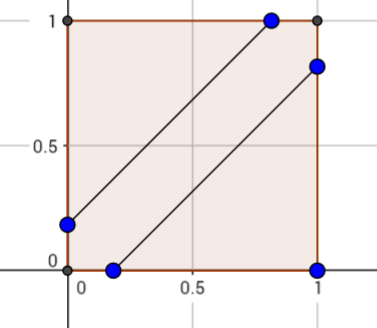
\includegraphics{2.png}

即两个边长是$\frac{2}{3}$的等腰直角三角形,和剩下的部分。虽然看起来面积不等,其实是相等的。让他们面积相等,是为了避免很多点都集中到了某个区域的情况,以及降低训练过程的难度。

接着我们令$O_2(0.5,0.5)$为中间部分的输出层结果,然后过他做两条直线的对称点$O_1,O_3$

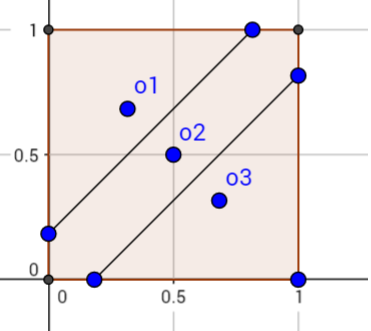
\includegraphics{1.png}

由于是对称点,所以两条直线分别成了$O_1O_2$和$O_2O_3$的垂直平分线。垂直平分线有个特性,即离某个点更近的所有点都集中在其中一侧。

这样子的话,在这个正方形中,离$O_1$最近的点就是左上角的三角形,面积$\frac{1}{3}$;离$O_2$最近的点就是中间的部分,面积$\frac{1}{3}$,离$O_3$最近的点就是右下角的三角形,面积$\frac{1}{3}$。

我们让$A$类数据的输出层期望输出点$O_1$,$B$类数据的输出层期望输出点$O_2$,$C$类数据的输出层期望输出点$O_3$。

训练完之后进行分类时,对每个数据的输出层找他离哪个点最近,就代表在哪一类。

分类正确率如下:

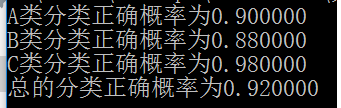
\includegraphics{3.png}

\end{document}
